\documentclass[11pt]{article}
\usepackage[utf8]{inputenc}

% --- Packages ---
\usepackage[usenames, dvipsnames]{color} % Cool colors
\usepackage{enumerate, amsmath, amsthm, amssymb, mathrsfs, algorithm, algpseudocode, fontawesome, pifont, subfig, fullpage, csquotes, dashrule, tikz, bbm, booktabs, bm, hyperref, wasysym}
\usepackage{blindtext, microtype, graphicx, wrapfig, enumitem, fancyhdr, index}
\usepackage[framemethod=TikZ]{mdframed}
\usepackage[numbers]{natbib}
\usepackage[normalem]{ulem}

% --- Misc. ---
\hbadness=10000 % No "underfull hbox" messages.
\setlength{\parindent}{0pt} % Removes all indentation.

% -- Commands --
% Dynamically sized mid bar.
\newcommand{\bigmid}{\mathrel{\Big|}}

% ---- Colors and Notes ----
% ---- Colors and Notes ----
\definecolor{dblue}{RGB}{98, 140, 190}
\definecolor{dmblue}{RGB}{169, 193, 219}
\definecolor{dlblue}{RGB}{216, 235, 255}
\definecolor{dred}{RGB}{195, 112, 113}
\definecolor{dorange}{RGB}{230, 169, 132}
\definecolor{dgreen}{RGB}{83, 127, 85}
\definecolor{dmgreen}{RGB}{118, 167, 125}
\definecolor{dlgreen}{RGB}{154, 195, 157}
\definecolor{dtan}{RGB}{221, 215, 200}
\definecolor{dpink}{RGB}{207, 166, 208}
\definecolor{dyellow}{RGB}{255, 248, 199}
\definecolor{dgray}{RGB}{46, 49, 49}

% Lights
\definecolor{dlblue}{RGB}{169, 193, 219}
\definecolor{dlgreen}{RGB}{154, 195, 157}
\definecolor{dyellow}{RGB}{246, 240, 223}


% URL
\newcommand{\durl}[1]{\textcolor{dblue}{\underline{\url{#1}}}}
\newcommand{\tx}[1]{\text{#1}}

% Circled Numbers
\newcommand*\circled[1]{\tikz[baseline=(char.base)]{\node[shape=circle,draw,inner sep=0.7pt] (char) {\footnotesize{#1}};}}
% From: http://tex.stackexchange.com/questions/7032/good-way-to-make-textcircled-numbers

% Under set numbered subset of equation
\newcommand{\numeq}[3]{\underset{\textcolor{#2}{\circled{#1}}}{\textcolor{#2}{#3}}}

\newcommand{\dnote}[1]{\textcolor{dblue}{Dave: #1}}

% ---- Abbreviations -----
\newcommand{\tc}[2]{\textcolor{#1}{#2}}
\newcommand{\ubr}[1]{\underbrace{#1}}
\newcommand{\uset}[2]{\underset{#1}{#2}}
\newcommand{\eps}{\varepsilon}
\newcommand{\KL}[2]{D_{\text{KL}}\left(#1 \mid \mid #2\right)}
\newcommand{\bKL}[2]{D_{\text{KL}}\left(#1 \bigmid \bigmid #2\right)}

% Typical limit:
\newcommand{\nlim}{\underset{n \rightarrow \infty}{\lim}}
\newcommand{\nsum}{\sum_{i = 1}^n}
\newcommand{\nprod}{\prod_{i = 1}^n}

% Add an hrule with some space
\newcommand{\spacerule}{\begin{center}\hdashrule{2cm}{1pt}{1pt}\end{center}}

% Mathcal and Mathbb
\newcommand{\mc}[1]{\mathcal{#1}}
\newcommand{\indic}{\mathbbm{1}}
\newcommand{\bE}{\mathbb{E}}

\newcommand{\longra}{\longrightarrow}
\newcommand{\longla}{\longleftarrow}
\newcommand{\ra}{\rightarrow}
\newcommand{\la}{\leftarrow}

% argmin, argmax.
\DeclareMathOperator*{\argmin}{arg\,min}
\DeclareMathOperator*{\argmax}{arg\,max}

% Quick Matrix.
\newcommand{\mat}[1]{\begin{bmatrix}#1\end{bmatrix}}

% ---- Figures, Boxes, Theorems, Etc. ----

% Basic Image
\newcommand{\img}[2]{
\begin{center}
\includegraphics[scale=#2]{#1}
\end{center}}

% Put a fancy box around things.
\newcommand{\dbox}[1]{
\begin{mdframed}[roundcorner=4pt, backgroundcolor=gray!5]
\vspace{1mm}
{#1}
\end{mdframed}
}

%  --- PROOFS ---

% Inner environment for Proofs
\newmdenv[
  topline=false,
  bottomline=false,
  rightline = false,
  leftmargin=10pt,
  rightmargin=0pt,
  innertopmargin=0pt,
  innerbottommargin=0pt
]{innerproof}

% Proof Command
%\newenvironment{dproof}{\begin{proof} \text{\vspace{2mm}} \begin{innerproof}}{\end{innerproof}\end{proof}\vspace{4mm}}
\newenvironment{dproof}[1][Proof]{\begin{proof}[#1] \text{\vspace{2mm}} \begin{innerproof}}{\end{innerproof}\end{proof}\vspace{4mm}}


% Dave Definition
\newcounter{DaveDefCounter}
\setcounter{DaveDefCounter}{1}

\newcommand{\ddef}[2]
{
\begin{mdframed}[roundcorner=1pt, backgroundcolor=white]
\vspace{1mm}
{\bf Definition \theDaveDefCounter} (#1): {\it #2}
\stepcounter{DaveDefCounter}
\end{mdframed}
}

% Block Quote
\newenvironment{dblockquote}[2]{
\begin{blockquote}
#2
\vspace{-2mm}\hspace{10mm}{#1} \\
\end{blockquote}}

% Algorithm
\newenvironment{dalg}[1]
{\begin{algorithm}\caption{#1}\begin{algorithmic}}
{\end{algorithmic}\end{algorithm}}

% Dave Table
\newenvironment{dtable}[1]
{\begin{figure}[h]
\centering
\begin{tabular}{#1}\toprule}
{\bottomrule
\end{tabular}
\end{figure}}

% For numbering the last of an align*
\newcommand\numberthis{\addtocounter{equation}{1}\tag{\theequation}}


\newtheorem{assumption}{Assumption}
\newtheorem{conjecture}{Conjecture}
\newtheorem{corollary}{Corollary}
\newtheorem{claim}{Claim}
\newtheorem{example}{Example}
\newtheorem{lemma}{Lemma}
\newtheorem{proposition}{Proposition}
\newtheorem{remark}{Remark}
\newtheorem{theorem}{Theorem}

\begin{document}
\title{CVPR 2019 Notes \\ \Large{Long Beach, CA, USA}}
\author{Shuai Chen \\ \durl{shuaic92@gmail.com}}
\date{June 2019}

\maketitle
\tableofcontents
\newpage

This documents contains notes I took during CVPR 2019 conference in Long Beach, CA, USA. My motivation of making this document came from the inspiration of David Abel\footnote{\durl{http://david-abel.github.io}}. Please feel free to distribute it as well as correcting my typos and mistakes. My email is \durl{shuaic92@gmail.com}.

\section{Conference Highlights}
This was my first time took part in such an awesome academic conference. Most of my time spent in Deep Learning \& Computational Photography related topics. However, I would also update some topics that I found interesting.
\begin{enumerate}
    \item Around 10,000 people attend this year's conference. About 1300 papers were accepted in CVPR 2019. Reports saying number of attendees projected in 2035 will be over 1 million :). See Figure \ref{fig:Conf_HL1}.
    \begin{figure}[h!]
        \centering
        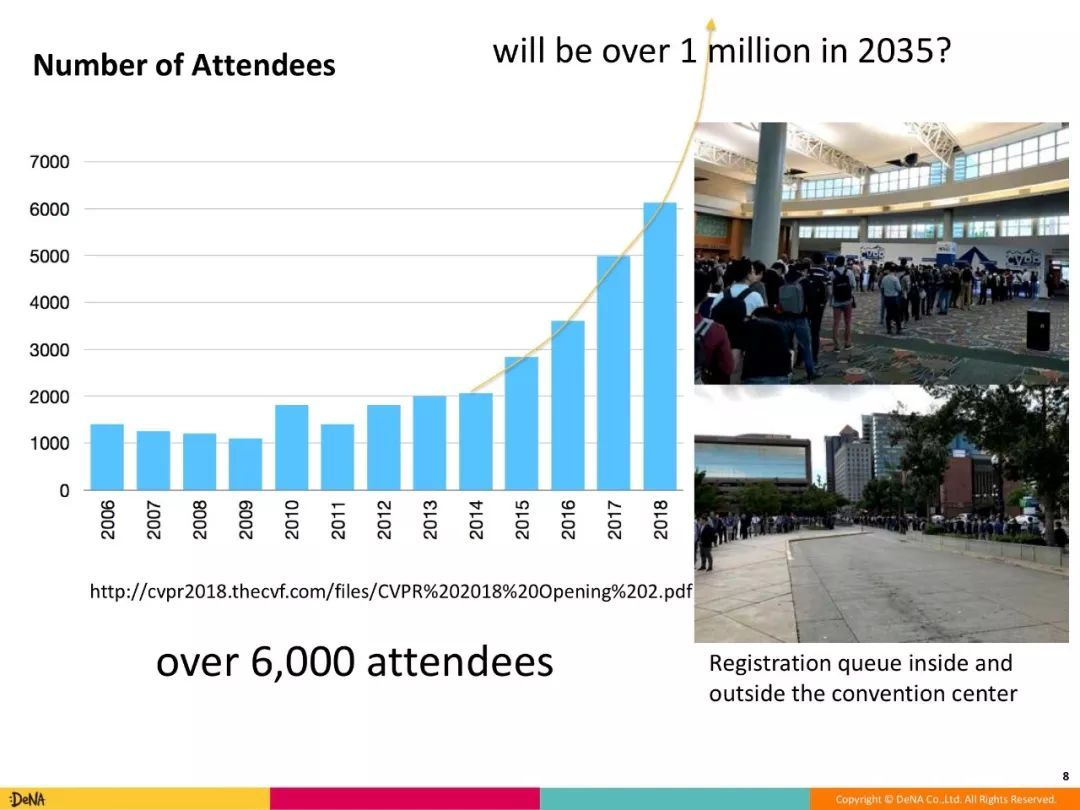
\includegraphics[width=0.5\textwidth]{images/Image1.jpeg}
        \caption{projection of attendees to reach 1 million by 2035}
        \label{fig:Conf_HL1}
    \end{figure}
    
    \item Comparing to last year, the number of papers accepted in CVPR 2019 increased about 30\%. However, due to the fact that the number of papers submitted this year has increased 56.2\%, thus the paper acceptance rate reduced 4\% this year. See Figure \ref{fig:Conf_HL2}.
    \begin{figure}[ht!]
        \centering
        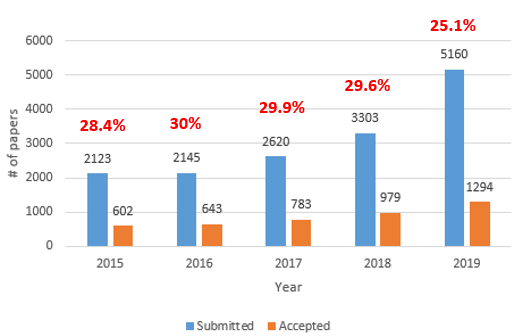
\includegraphics[width=0.5\textwidth]{images/Image2.png}
        \caption{papers acceptance rate is 4\% lower in CVPR 2019}
        \label{fig:Conf_HL2}
    \end{figure}
    
    \newpage
    \item Some of hot keywords in CVPR 2019 submission: Image, detection, 3d, object, video, segmentation, adversarial, recognition, visual. See Figure \ref{fig:Conf_HL3}
    \begin{figure}[ht!]
        \centering
        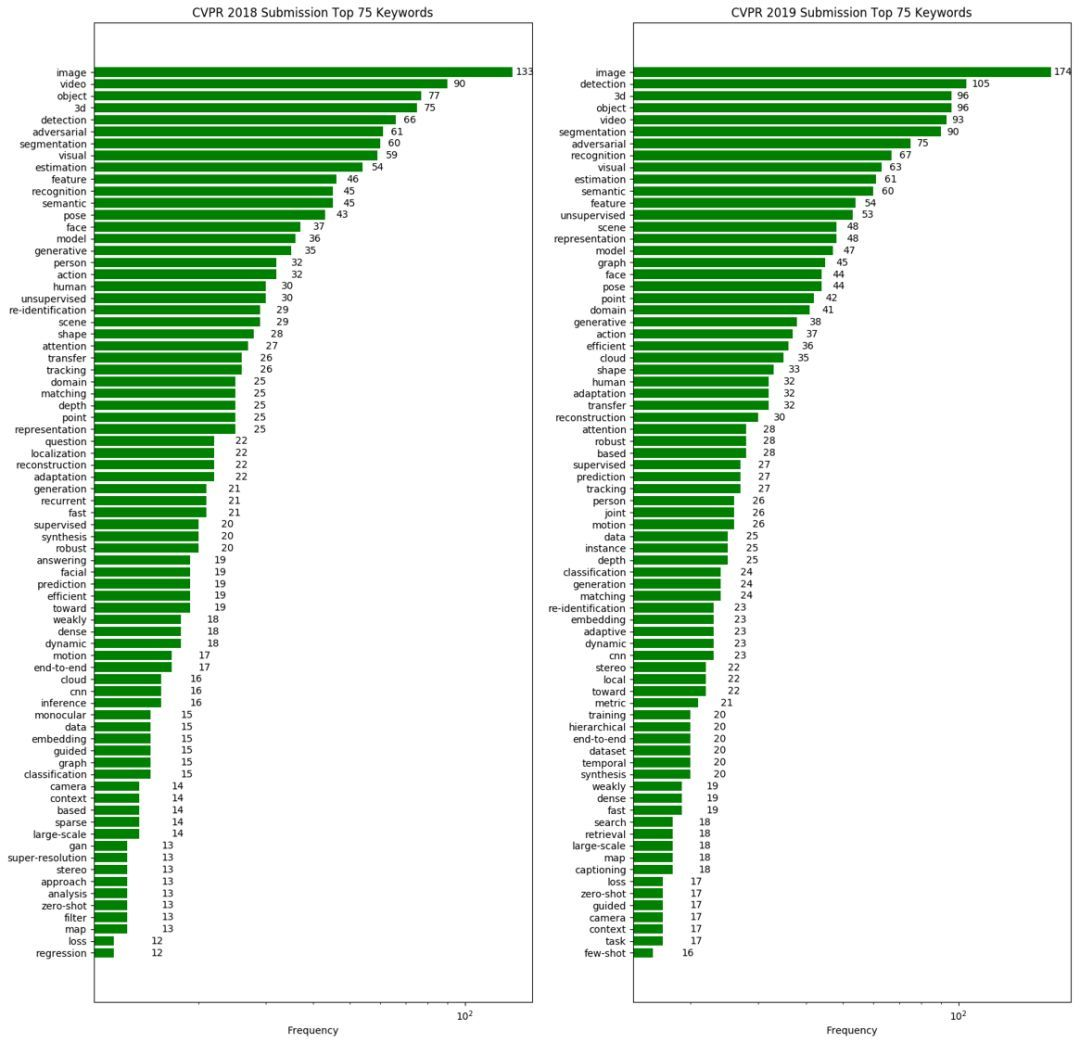
\includegraphics[width=0.9\textwidth]{images/Image3.jpeg}
        \caption{hot submission keywords CVPR 2018 vs. CVPR 2019}
        \label{fig:Conf_HL3}
    \end{figure}
    
    \item Meta-learning, One-shot/Few-shots learning, Graph Neural Networks started to emerging this year.
    \item It's great to see a lot of fast pace improvement towards real-life low level image processing field.
    \item Network Architecture Search is also another very popular topic. Great to see a burst of diverse solutions in this field.
    \item Generative Adversarial Network is a hot topic again. Exciting progress were made again this year.
\end{enumerate}{}

% ------------
% -- Sunday --
% ------------
\newpage
\section{Sunday June 16th: Tutorials \& Workshops}
Caught up part of Deep-Vision workshop. I was a little bit confused on overwhelming tutorials and workshops. I also spent a lot of time trying to find the correct room. So first day's note was not really good. Please feel free to contact me and add some notes.

\subsection{Workshop: Deep-Vision}
\subsubsection{Topic: AI on Medicine, Speaker: Serena Yeung}
Arrived at the end of the talk on this topic. She talked about Learning from few labeled training examples \\
\textbf{Learning to learn from noisy web videos (CVPR2017)}\newline
{\bf Idea:} Proposed a Reinforcement learning-based method for learning data labeling form noisy web videos. Result is able to learn domain-specific knowledge, and label data for new classes while avoiding semantic drift.\\
\\
\begin{figure}[]
    \centering
    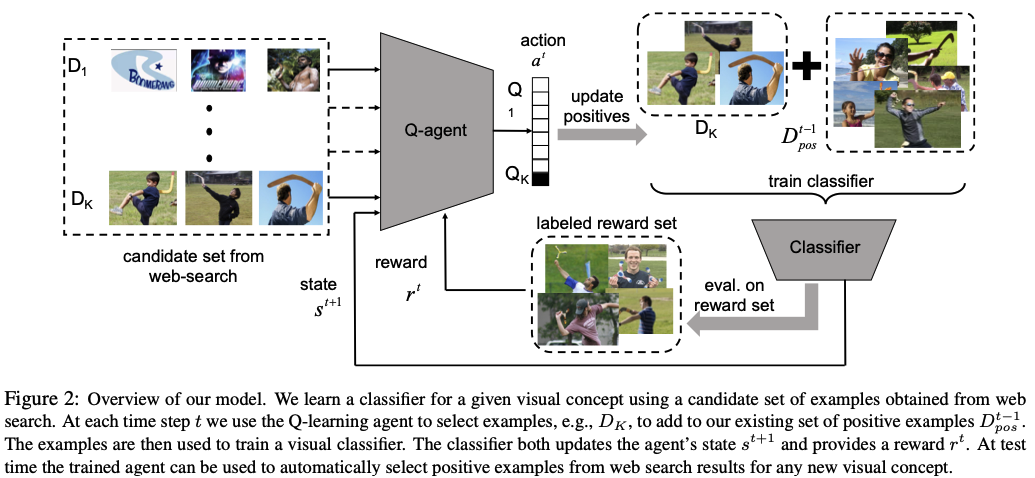
\includegraphics[width=1\textwidth]{images/Image4.png}
    \label{fig:Conf_D1_1}
\end{figure}\\
{\bf Terminology:} \textit{candidate set:} noisy search result. \textit{reword set:} a set of examples annotated with the presence or absence of the target class.\\
\\
\textbf{Temporal Modular Networks for Retrieving Complex Compositional Activities in Videos (ECCV2018)}\\
\\
\textbf{Neural Graph Matching Networks for Fewshot 3D Action Recognition (ECCV2018)}\\
\\
Talked about Towards full realization of an AI-assisted hospital: Integration of multimodal data sources. \\
Talked about Jointly Learning Energy Expenditures and Activities using Egocentric Multimodal Signals (CVPR 2017) \\
Will add a short paper summary here... \\

\subsubsection{Topic: Video Re-Id, Speaker: Prof. Dr. Laura Leal-Taixé}
Tractor++ (reId+CMC)\\
CMC = motion camera model
\subsubsection{Topic: Video Super-resolution, Speaker: Prof. Dr. Laura Leal-Taixé}
Designed new Temporal Loss to improve video SR performance. Great results.
\subsubsection{Topic: Google Brain Pierre Sermanet: Self-Supervision and Play}
-Label Free\\
-Time-Contrastive Networks (TCN)\\
-Object-contrastive Networks\\



\end{document}